\documentclass[journal]{IEEEtran}
\usepackage{amsmath,amssymb,booktabs,graphicx,url}
\usepackage{tikz}
\usetikzlibrary{positioning,arrows.meta}
\newcommand{\pending}[1]{\textbf{[Pending evidence: #1]}}
\title{Transformation-Aware Persistent Derived-Data Reuse for Evolving Machine-Learning Pipelines}
\author{\pending{Author names, affiliations, and ORCID}}
\begin{document}
\maketitle
\begin{abstract}
Deterministic input preprocessing can recur across training epochs and related experiments even when most derived results remain valid. Materialized datasets remove repeated computation but leave applications responsible for identifying reusable artifacts as sources and transformations evolve. This manuscript studies Aether, a research prototype combining source and transformation identity with an immutable persistent artifact store implemented through a Java storage engine. A Python client constructs artifact keys, retrieves existing results, and lazily publishes missing outputs. The evaluation protocol pairs repeated preprocessing, Aether, an incremental memory-mapped baseline, and a memory-resident reference. It separates initial population from subsequent training, checks tensor and final-model parity, measures loader and client concurrency, and injects process failures at publication boundaries. The confirmatory performance evaluation and cross-dataset results remain pending. Consequently, this draft describes the implemented system and reproducible methodology without asserting a throughput advantage, performance equivalence, or submission readiness.
\end{abstract}
\begin{IEEEkeywords}
Persistent caching, derived data, parallel input pipelines, incremental reuse, performance evaluation.
\end{IEEEkeywords}

\section{Introduction}
Input preprocessing can compete with model execution for the resources required to sustain a training job. Repeating a deterministic transformation does not necessarily produce new information: if its source content and configuration are unchanged, its previous result may be reusable. The relevant systems problem extends beyond retaining bytes. A persistent artifact must have an identity that distinguishes incompatible transformations, a publication protocol that prevents partial visibility, and an access path whose cost can be measured against a specialized materialized representation.

Existing systems already accelerate input pipelines. FFCV combines a specialized storage format with caching, preloading and compilation~\cite{ffcv}; DALI provides an optimized processing runtime~\cite{dali}. HyCache considers partial caching of intermediate outputs across memory and storage~\cite{hycache}. Seneca studies cache partitioning and sampling for concurrent jobs~\cite{seneca}. Aether therefore makes no claim to invent preprocessing caches. Its research question is whether explicit persistent artifact identity can support safe reuse across dataset and pipeline evolution at a small cost relative to a workload-specific persistent baseline.

This draft separates implemented mechanisms from claims requiring measurement. The implemented mechanisms include deterministic client-side artifact keys, a Java-engine storage path, immutable publications, a true mmap baseline, paired experiment orchestration, and correctness and process-crash tests. The planned empirical contributions require completed remote measurements: reuse selectivity, training benefit relative to recomputation, abstraction overhead relative to mmap, and behavior under concurrent access. \pending{Replace this paragraph with evidence-backed contributions after protocol and statistical freeze.}

\section{Problem Formulation and Related Work}
Let a deterministic pipeline configuration be $p$, a sample identity be $s$, and its verified content digest be $h_s$. A derived artifact key is a digest of a canonical descriptor containing $s$, $h_s$, and the parameters and implementation version of $p$. A matching key is eligible for reuse; a changed descriptor produces a different lookup. The client forms this descriptor, while the Java engine owns persistent lookup, publication and storage. The engine does not independently reconstruct the source or execute arbitrary preprocessing code to verify the descriptor.

The application must version changes that affect semantics. Stochastic augmentation remains outside the cached segment; reproducible randomness would otherwise have to participate in identity. Hash identity assumes correct canonicalization and a collision-resistant digest. The cache is not evaluated as a security boundary against malicious producers.

The current artifact contains final pipeline outputs. Changing the normalization scale, output size, artifact codec or pipeline version invalidates the final artifact. No claim of reuse of upstream intermediate stages follows from this behavior. FFCV and DALI address execution and delivery efficiency; HyCache and Seneca also address caching decisions and sharing~\cite{ffcv,dali,hycache,seneca}. A full comparative evaluation must preserve each workload's tensor semantics and explicitly identify any unsupported operator or representation. \pending{Add equivalent external baseline measurements or a measured semantic compatibility audit.}

\section{Aether Design}
\subsection{Identity and Lookup}
The benchmark verifies source hashes before timing. Its descriptor includes sample identity, source identity and content, deterministic preprocessing parameters, normalization scale and offset, and an explicit pipeline version. The descriptor is encoded canonically and hashed. The resulting digest becomes the sample component of a Java cache key inside a workload namespace. A batched miss triggers deterministic preprocessing and serialization; a hit bypasses that computation.

\begin{figure}[t]
\centering
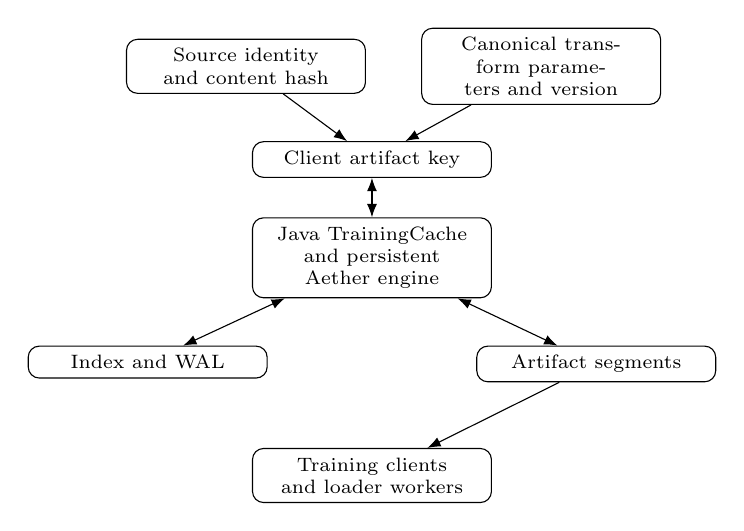
\begin{tikzpicture}[node distance=5mm, every node/.style={draw,rounded corners,align=center,text width=28mm,font=\scriptsize}, >=Latex]
\node (src) {Source identity and content hash};
\node[right=7mm of src] (transform) {Canonical transform parameters and version};
\node[below=6mm of src,xshift=16mm] (key) {Client artifact key};
\node[below=of key] (java) {Java TrainingCache and persistent Aether engine};
\node[below left=6mm and -2mm of java] (index) {Index and WAL};
\node[below right=6mm and -2mm of java] (data) {Artifact segments};
\node[below=19mm of java] (workers) {Training clients and loader workers};
\draw[->] (src)--(key); \draw[->] (transform)--(key);
\draw[<->] (key)--(java); \draw[<->] (java)--(index); \draw[<->] (java)--(data);
\draw[->] (data)--(workers);
\end{tikzpicture}
\caption{Implemented derived-data path. The client binds source and transform identity; the Java engine owns persistent storage. Miss computation occurs in the client-side deterministic pipeline.}
\label{fig:architecture}
\end{figure}

\subsection{Publication and Lifecycle}
Cache keys are immutable: repeated matching publications are idempotent and conflicting payloads are rejected. Batch publication validates keys before modifying persistent state and encodes each new artifact once. Large values are written into uniquely named temporary files, forced in durable mode, and atomically renamed before committing their index metadata. On the Linux code path, directory synchronization precedes the durable index commit. Windows process-crash tests do not establish identical directory persistence behavior.

Dataset removal does not imply immediate deletion of old artifacts. V2 accesses its own active identities; retained V1 entries remain storage overhead until eviction or lifecycle maintenance. The acknowledged-write contract is tested below configured capacity and without intentional namespace invalidation. Capacity eviction is a separate semantic event and must not be mistaken for crash-related loss.

\subsection{Parallel Access}
Training loader workers own independent client connections and mapping handles. First-epoch publication is completed before scheduling the next epoch, preventing speculative next-epoch reads from changing expected first-miss counts. Worker startup and epoch transitions are included in measured wall time. Independent client processes share a Java daemon or a locked persistent mmap store in a separate storage benchmark. Concurrent clients may perform duplicate preprocessing before observing another publication; client publication attempts are not reported as unique engine commits.

\section{Implementation}
The Java module uses the repository's persistent Aether engine. A binary loopback protocol supports batched reads and writes; an information request verifies the actual engine and durability mode before measurements. Python orchestrates preprocessing and PyTorch execution and does not substitute a Python artifact index in the Java benchmark.

The specialized baseline stores framed tensor payloads in an append-only data file. Reads use read-only mmap slices. Index batches are appended to a checksummed journal after the corresponding data is synchronized in durable mode; publication does not rewrite the entire index. Recovery ignores incomplete journal tails and rejects complete records with invalid checksums. Missing samples are appended in batches, and payload checksums and framing are verified on reads. Mapping lifetime is explicitly bounded on Windows when processes share a writable store.

OCT inputs use the existing deterministic segmentation pipeline. RGB workloads use verified image manifests, RGB decoding, bilinear resizing, optional Gaussian passes and fixed normalization. COCO labels encode image-level object-category presence; ImageNet labels encode one class. This is a classification systems workload, not an object-detection accuracy evaluation. All backends reconstruct the same fp32 model inputs from the same fp16 artifact representation.

\section{Experimental Methodology}
\subsection{Datasets and Workload Semantics}
OCT5k provides multi-grader retinal annotations for 1672 OCT scans~\cite{oct5k}. The source dataset includes segmentation and biomarker annotations; this experiment uses its deterministic segmentation input path as a systems workload. COCO provides heterogeneous natural images and instance annotations~\cite{coco}; the implemented adapter reduces object categories to image-level presence labels for a multi-label classification workload. ImageNet uses the classification dataset associated with ILSVRC~\cite{imagenet}. These task adaptations define the benchmark inputs and do not reproduce the datasets' original detection or challenge accuracy evaluations. The exact selected releases, annotation choices, cardinalities and manifest hashes must accompany the measured tables.

\subsection{Primary Protocol}
The frozen primary OCT evolution has 1170 V1 samples and 1505 V2 samples, with 1003 reusable identities. Ten V2 epochs imply 15050 lookups, 14548 hits and 502 misses when every sample is seen once per epoch. These are invariants to verify, not recorded experimental outcomes. Each paired block independently populates V1 in Java and mmap stores, restarts Java, and measures the four backends in a seeded randomized order. The confirmatory plan fixes exactly 24 fresh independent blocks, batch size 16, prefetch depth zero, server tracing off, asynchronous compaction on, and checksum policy \texttt{immutable-inline-admission-v1}. All pilot measurements are excluded.

\subsection{Timing and Resource Accounting}
Effective throughput is processed training samples divided by measured training wall time. The reports separately retain population cost, command wall time, input waiting, lookup and publication timing, bytes, GPU sampling and process metrics. Reference preparation and source/presence verification precede measurement and can warm the OS page cache. The Kaggle protocol therefore makes no cold-cache storage claim. Unsupported per-mapping page-fault attribution is recorded as unavailable. Full-reference and RAM-baseline memory requirements limit feasible dataset cardinality.

Large-cardinality runs may omit the RAM reference while retaining the RAW, Java and mmap comparison; reference tensors are then generated with bounded memory. Both persistent stores can occupy a configured scratch filesystem while reports remain in the saved results directory. Before a block, the runner checks a payload capacity lower bound and records free space. This check is not a disk reservation or a complete estimate of index and transient-write overhead. Insufficient capacity stops the specified experiment rather than changing its sample count. The source/runtime build receipt, frozen environment and exclusive output lock prevent accidental reuse of stale Java binaries or simultaneous writers to one campaign's evidence.

\subsection{Canonical DALI Comparison}
The secondary RGB comparison uses a separate canonical pipeline: DALI mixed-device RGB decoding, antialiased bilinear resizing and fixed normalization to CHW fp16 outputs~\cite{dali}. The direct baseline delivers GPU tensors to PyTorch through DLPack with prefetch enabled. The Java and mmap backends cache outputs of the same DALI operators; misses execute those operators on demand. Canonical payload hashes and exact final-model equality are mandatory. This design avoids assuming that Pillow and DALI decoding or interpolation produce identical tensors. The secondary protocol, software environment and analysis are separate from the primary experiment. CUDA runtime validation and the twelve paired repetitions per dataset remain pending.

\subsection{Statistics}
The sole primary hypothesis is throughput equivalence to pre-materialized mmap over all ten V2 training epochs. Effective throughput divides the 15050 processed samples by total V2 training wall time, including inline Aether admission but excluding V1 population, mmap pre-materialization, reference validation, daemon startup and the post-training compaction drain. For each block, the analysis computes log Aether/mmap throughput ratios and performs two one-sided tests at $\alpha=0.05$. Equivalence requires the exponentiated Student-$t$ 90\% confidence interval to lie strictly inside 0.97--1.03. The secondary RAW comparison is a one-sided paired log-ratio superiority test at $\alpha=0.05$; it does not change the primary decision. RAM is descriptive. Cumulative epoch 1--10 costs from the same blocks are a secondary amortization analysis, with no endpoint selection. Additional 95\% intervals, paired bootstrap and Wilcoxon analyses are sensitivity summaries. Failure to detect a difference is not evidence of equivalence.

Protocol, environment and condition identifiers prevent pooling heterogeneous replicas. Raw-report hashes and invariant checks guard the analysis input. Secondary worker, reuse, cost and size campaigns have separate interpretation; an optional mixed-effects model treats paired blocks as random intercepts. Normal-approximation planning is not a guarantee of equivalence-test power.

\subsection{Correctness and Failures}
The artifact checks exact tensor parity and final model-state parity under deterministic execution. Source, normalization, resize, implementation-version and lossless artifact-codec evolution are tested against persistent Java and mmap stores. Failure injection externally terminates the Java process before data write, after data synchronization, before index commit, after index commit before API return, and after the caller observes return. Recovery verifies visible checksums, acknowledged records, orphan bytes and elapsed reopen time. The full plan calls for 100 repetitions at every point for both single and batch publication. Process termination is distinct from power interruption.

\section{Evaluation}
\pending{Import measured hardware/software table, 24-block primary results, two additional datasets, reuse/cost/size sweeps, loader/client/GPU scaling, and full failure campaign.}

Figures and tables are generated from validated raw blocks by \texttt{scripts/figures.py}; throughput and ratios use measured aggregates and confidence intervals. The draft intentionally contains no fabricated bars, zero-valued result placeholders, or reused single-run preliminary claims. CPU smoke measurements verify implementation behavior and are excluded from the GPU performance dataset.

\section{Discussion and Limitations}
The evaluation is presently single-node. Two-GPU DataParallel execution does not establish distributed scaling. The concurrent storage microbenchmark and GPU loader experiment measure different effects and must be interpreted separately. Persistent identity provides safe misses only when producers supply correct source digests and version their transformation semantics. Final-artifact caching does not establish selective intermediate-stage reuse. OS page-cache warming, full-reference memory consumption, index-journal publication cost and client transport overhead remain relevant experimental factors.

OCT data are used solely for systems evaluation. No throughput result implies clinical efficacy. Dataset licenses and access restrictions govern acquisition and sharing; the artifact distributes preparation code and manifests rather than source images. GPU resource usage and any available energy measurements must accompany the final evaluation. \pending{Record actual GPU-hours and any available measured energy, with measurement boundaries.}

\section{Conclusion}
This draft specifies and implements a persistent derived-data evaluation path through the Java Aether engine. Its empirical claims remain conditional on completed, frozen and independently reproducible measurements. The principal question is the cost and correctness of explicit derived-artifact identity across evolution, rather than whether caching itself is novel.

\section*{Acknowledgment}
\pending{Author review of disclosure. OpenAI Codex assisted with software implementation, test development, artifact organization and manuscript drafting. Describe the retained material and actual author verification before submission; do not claim verification that has not occurred.}
\bibliographystyle{IEEEtran}
\bibliography{references}
\end{document}
